\documentclass[conference]{IEEEtran}
\usepackage[T1]{fontenc}
\usepackage{amsmath}
\usepackage{booktabs}
\usepackage{tabularx}
\usepackage{tikz}
\usetikzlibrary{arrows.meta,positioning}

\title{Real-Time OS Resource Governance and Deadlock Avoidance for Edge Computing in Intelligent Transportation Systems (SDG 11)}

\author{\IEEEauthorblockN{Smart Traffic OS Research Team}
\IEEEauthorblockA{NIET Operating Systems Project\\
Smart Traffic Management System}}

\begin{document}
\maketitle

\begin{abstract}
Intelligent transportation systems (ITS) combine signal control, camera
analytics, public transport, and emergency response on resource-constrained
edge platforms. These workloads contend for processor time, memory, and shared
intersection resources. This paper presents a teaching-oriented operating
system simulation that connects real-time scheduling, process-state tracking,
deadlock prevention, memory replacement, and edge isolation to Sustainable
Development Goal 11. The prototype models an extended process control block,
Preemptive Priority, Round Robin, and multilevel feedback queue (MLFQ)
scheduling with a 0.2 ms context-switch penalty, monotonic lock acquisition,
the Priority Ceiling Protocol, and Banker's safety analysis. It also evaluates
FIFO, LRU, LFU, and Optimal page replacement and demonstrates raw-frame
transport through POSIX shared memory. On the repository's four-task master
workload, Preemptive Priority records 4.25 ms average waiting time (AWT) and
7.75 ms average turnaround time (ATAT); the corresponding MLFQ and Round Robin
values are 6.30/9.80 ms and 6.70/10.20 ms. Page-fault percentages on the
20-reference, three-frame master benchmark are 85%, 90%, 70%, and 55% for
FIFO, LRU, LFU, and Optimal, respectively. All reported timing values are
simulated, not kernel real-time guarantees or measurements from deployed
traffic infrastructure.
\end{abstract}

\begin{IEEEkeywords}
Real-Time Kernels, MLFQ, Priority Ceiling Protocol, Banker's Algorithm, Edge
Computing, Intelligent Transportation Systems, SDG 11
\end{IEEEkeywords}

\section{Introduction and Urban Traffic Bottlenecks}
Urban traffic infrastructure is a distributed cyber-physical system. Signal
controllers, cameras, connected vehicles, public transport, and emergency
services compete for CPU, memory, and synchronization resources. An operating
system (OS) must balance emergency response with fair service, avoid deadlock
on shared resources, and contain interference among edge workloads.

This project frames those concerns as OS mechanisms: vehicles and analytics
jobs are processes, intersection zones are shared resources, and camera frames
are memory and inter-process communication workloads. The motivation aligns
with SDG 11's emphasis on inclusive, safe, resilient, and sustainable cities.
The implementation is a Python user-space simulator and educational prototype;
it is not a safety-certified traffic controller. In particular, its simulated
times do not establish hard real-time deadlines.

\section{Related Work and Research Graph Synthesis}
Classical real-time scheduling analyzes how task priorities and execution
budgets affect response and deadline behavior~\cite{liu1973}. Priority
inheritance and ceiling protocols address priority inversion when real-time
tasks share resources~\cite{sha1990}. Operating-system texts treat safe-state
resource allocation, virtual-memory replacement, and process control blocks as
complementary resource-governance mechanisms~\cite{silberschatz2018}. The
working-set and replacement literature motivates comparing page faults under
different locality policies~\cite{belady1966}.

The synthesis graph in Fig.~\ref{fig:research-graph} connects these established
mechanisms to the project rather than claiming a systematic literature
database export. Scheduling governs dispatch latency; synchronization governs
shared-resource safety; virtual memory and shared memory govern camera-data
movement; and container controls address edge-service interference. Together,
these mechanisms motivate the measurable resilience outcomes studied here.

\begin{figure*}[t]
\centering
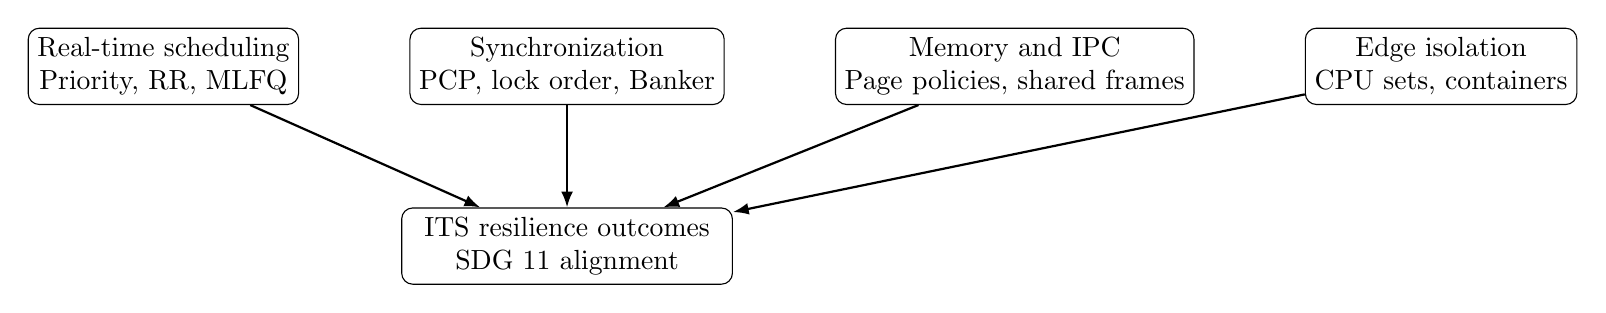
\begin{tikzpicture}[
  concept/.style={draw,rounded corners,align=center,minimum width=2.6cm,
    minimum height=0.85cm},
  link/.style={-{Latex[length=2mm]},thick},
  node distance=1.3cm and 1.4cm
]
\node[concept] (sched) {Real-time scheduling\\Priority, RR, MLFQ};
\node[concept,right=of sched] (sync) {Synchronization\\PCP, lock order, Banker};
\node[concept,right=of sync] (memory) {Memory and IPC\\Page policies, shared frames};
\node[concept,right=of memory] (edge) {Edge isolation\\CPU sets, containers};
\node[concept,below=of sync,minimum width=4.2cm] (sdg) {ITS resilience outcomes\\SDG 11 alignment};
\draw[link] (sched) -- (sdg);
\draw[link] (sync) -- (sdg);
\draw[link] (memory) -- (sdg);
\draw[link] (edge) -- (sdg);
\end{tikzpicture}
\caption{Research-topic synthesis linking OS resource mechanisms to ITS
resilience goals.}
\label{fig:research-graph}
\end{figure*}

\section{System Architecture and Extended PCB Design}
The prototype is organized into process management, scheduling, concurrency,
memory, telemetry, and deployment modules. The extended process control block
(PCB) stores a process identifier, thread-group identifier, lifecycle state,
priority, arrival and burst times, remaining execution, scheduling metrics,
CPU affinity, and simulated RIP/RSP/CR3/FLAGS register context. Its five-state
lifecycle is NEW, READY, RUNNING, WAITING, and TERMINATED.

The scheduler consumes PCB workloads and emits dispatch traces, process
metrics, and aggregate timing. The concurrency layer models three ordered
intersection zones, a priority-ceiling mutex, and Banker-style resource
admission. The memory layer implements page-replacement policies and a
POSIX-style shared-memory frame buffer. Telemetry renders Gantt and memory
benchmark charts. Docker Compose describes a possible service-isolation
deployment; it does not turn the Python scheduler into a kernel scheduler.

\section{Empirical CPU Scheduling and Context-Switch Overhead Analysis}
The engine compares Preemptive Priority, Round Robin, and a three-level MLFQ.
The MLFQ uses Round Robin quanta of 2 ms and 4 ms for its first two levels and
FCFS at the third level; lower queues are promoted after more than 15 ms of
waiting. Numeric priority 0 represents the highest scheduling priority.

For each change in selected process identifier, the simulation adds
$C_{sw}=0.2$ ms. If $N_{sw}$ is the number of process changes, the modeled
switch overhead is $T_{sw}=N_{sw}C_{sw}$. This is an explicit simulation
parameter, not an observed hardware cost. A separate response-time or
deadline guarantee would require measurements and analysis on the target
kernel and edge hardware.

\section{Deadlock Elimination and Monotonic Lock Hierarchies}
The intersection model orders zones as $Z_1<Z_2<Z_3$ and requires acquisition
in strictly increasing order and release in reverse. This removes circular
wait from the modeled lock graph. The Priority Ceiling Protocol raises a
lock owner's effective priority to the resource ceiling and restores its
original priority on release. The project's mutex is a single-resource
simulation; it does not implement expiring lock leases or a kernel PCP.

For resource allocation, the Banker adapter computes
$Need=Max-Allocation$ and accepts a tentative request only when a safe
completion sequence remains. Unsafe requests are rolled back. These
mechanisms address distinct risks: lock ordering prevents circular wait,
priority ceilings mitigate priority inversion, and Banker's analysis avoids
unsafe resource states.

\section{Zero-Copy Shared Memory and Page Replacement Evaluation}
The frame-transfer prototype uses Python's POSIX shared-memory interface to
place a length-prefixed raw frame in a shared mapping. On Linux, POSIX shared
memory is commonly backed by \/dev\/shm. This avoids an additional pipe or
socket payload transfer in the modeled producer-consumer path, but the
prototype does not claim zero-copy behavior through every camera, driver, or
inference-library stage.

FIFO, LRU, LFU, and Optimal replacement are evaluated against the same
20-reference master workload with three frames. The fault percentage is
$100F/R$, where $F$ is the number of page faults and $R$ is the number of
references. Optimal is a theoretical lower-bound policy because it assumes
knowledge of future references.

\section{Experimental Results and Discussion}
Table~\ref{tab:scheduling} reports the master scheduler metrics. The AWT and
ATAT values are copied from the repository's executable master workload.
Table~\ref{tab:pages} reports the corresponding page-fault counts and
percentages. These are deterministic simulator results and should be
interpreted only for the stated workloads and parameters.

\begin{table*}[t]
\caption{CPU Scheduling Results for the Master Workload}
\label{tab:scheduling}
\centering
\begin{tabular}{lrrrr}
\toprule
Scheduler & AWT (ms) & ATAT (ms) & ART (ms) & Throughput \\
\midrule
Preemptive Priority & 4.25 & 7.75 & 2.60 & 0.2703 \\
3-Tier MLFQ & 6.30 & 9.80 & 1.80 & 0.2632 \\
Round Robin & 6.70 & 10.20 & 2.35 & 0.2597 \\
\bottomrule
\end{tabular}
\end{table*}

\begin{table}[t]
\caption{Page-Replacement Results (20 References, 3 Frames)}
\label{tab:pages}
\centering
\begin{tabular}{lrrr}
\toprule
Policy & Faults & Hits & Faults (\%) \\
\midrule
FIFO & 17 & 3 & 85.00 \\
LRU & 18 & 2 & 90.00 \\
LFU & 14 & 6 & 70.00 \\
Optimal & 11 & 9 & 55.00 \\
\bottomrule
\end{tabular}
\end{table}

Preemptive Priority has the lowest AWT among these three runs, while MLFQ has
the lowest reported average response time (ART). The result is workload
dependent: the metrics do not establish that one policy dominates under all
arrival patterns. LRU's 90\% fault ratio exceeding FIFO's 85\% also illustrates
that replacement policy performance depends on the reference sequence; the
Optimal row is a future-aware bound, not an implementable online policy.

\section{Conclusion and Future Directions}
This work combines scheduler metrics, PCB state, lock-order enforcement, PCP,
safe-state resource admission, shared-memory transport, and page-replacement
benchmarks in an ITS-oriented OS simulation. The results make tradeoffs
reproducible and connect OS mechanisms to SDG 11 resilience objectives without
claiming field deployment or hard real-time behavior.

Future work includes adding validated literature references and target-device
measurements, testing scheduler behavior under real Linux real-time policies,
measuring end-to-end camera latency, adding lease-aware synchronization and
watchdogs, and evaluating the system on an isolated edge testbed. Physical
traffic control would require independent safety engineering, hazard analysis,
certified hardware interfaces, and fail-safe validation.

\begin{thebibliography}{00}
\bibitem{liu1973} C. L. Liu and J. W. Layland, ``Scheduling algorithms for
multiprogramming in a hard-real-time environment,'' \emph{Journal of the ACM},
vol. 20, no. 1, pp. 46--61, Jan. 1973.
\bibitem{sha1990} L. Sha, R. Rajkumar, and J. P. Lehoczky, ``Priority
inheritance protocols: An approach to real-time synchronization,''
\emph{IEEE Transactions on Computers}, vol. 39, no. 9, pp. 1175--1185,
Sep. 1990.
\bibitem{silberschatz2018} A. Silberschatz, P. B. Galvin, and G. Gagne,
\emph{Operating System Concepts}, 10th ed. Hoboken, NJ, USA: Wiley, 2018.
\bibitem{belady1966} L. A. Belady, ``A study of replacement algorithms for a
virtual-storage computer,'' \emph{IBM Systems Journal}, vol. 5, no. 2,
pp. 78--101, 1966.
\end{thebibliography}

\end{document}
